\documentclass[11pt,a4paper]{article}
\usepackage[utf8]{inputenc}
\usepackage[T1]{fontenc}
\usepackage{lmodern}
\usepackage[margin=2.5cm]{geometry}
\usepackage{amsmath,amssymb}
\usepackage{booktabs}
\usepackage{graphicx}
\usepackage{hyperref}
\usepackage{xurl}
\usepackage{setspace}
\onehalfspacing

\hypersetup{
    colorlinks=true,
    linkcolor=blue,
    citecolor=blue,
    urlcolor=blue
}

\title{\textbf{From Gold Standard to the Euro: Global Currency Blocs, Bretton Woods Realignments, and Floating Regimes, 1870--2013}}

\author{Petr Avtonomov\thanks{Independent Researcher, St.~Petersburg, Russia. ORCID: \href{https://orcid.org}{0009-0003-2816-6782}. Code and data repository: \url{https://github.com/avtonomov-petr/From-Gold-Standard-to-the-Euro}.}}
\date{November 2026}

\begin{document}

\maketitle

\begin{abstract}
In four preceding studies of early modern and nineteenth-century market integration, we audited Atlantic grain prices (\href{https://doi.org}{Avtonomov, 2026a}), Baltic Sound Toll shipping (\href{https://doi.org}{Avtonomov, 2026b}), St.~Petersburg--European exchange rates (\href{https://doi.org}{Avtonomov, 2026c}), and the Eurasian silver corridor (\href{https://doi.org}{Avtonomov, 2026d}) using singular value decomposition (SVD) and normalized participation ratios ($\mathrm{PR}$). Before extending this diagnostic apparatus to twenty-first-century geopolitical fractures, this fifth study provides a formal calibration benchmark across four well-documented international monetary regimes over \texttt{1870--2013} ($T = 144$ years): the classical gold standard (\texttt{1871--1913}), the interwar Great Depression (\texttt{1919--1939}), the Bretton Woods peg (\texttt{1946--1971}), and the post-Bretton Woods float (\texttt{1973--2013}). Evaluating all $N = 21$ economies with at least 90\% continuous annual coverage in the Clio Infra \emph{Exchange Rates to UK Pound} dataset (re-anchored to the US dollar and cross-checked directly against sterling), we confirm that the diagnostic cleanly separates diffuse, shock-driven, and institutional currency regimes. Under the classical gold standard, low shared variance ($\mathrm{Var}_1 = 27.0\%$) reflects tight specie-point stability around fixed parities; during the interwar crisis, shared variance surged ($\mathrm{Var}_1 = 46.8\%$) across broad cross-sections ($\mathrm{PR}(v_1) = 0.735$) punctuated by the 1920 deflation (26.4\%) and 1932--1934 gold-bloc breakup (37.5\%). Under Bretton Woods, fixed pegs compressed annual movement into a single step realignment ($\mathrm{PR}(u_1) = 0.060$ in USD; $0.008$ in GBP), with 75.2\% of Mode~1 energy concentrated in the 1949--1950 European devaluations. Finally, in the post-1973 float, Mode~1 ($\mathrm{Var}_1 = 35.6\%$) isolates the 1999 Euro launch ($\mathrm{PR}(u_1) = 0.043$, 59.7\% temporal energy), where the top seven future Eurozone contributors account for 73.7\% of spatial variance (90.8\% in GBP), while orthogonal Mode~2 ($\mathrm{Var}_2 = 17.6\%$) captures Latin American debt crises.
\end{abstract}

\noindent\textbf{Keywords:} international monetary history, gold standard, Bretton Woods, Eurozone, exchange rate regimes, cliometrics, spectral analysis, participation ratio.

\section{Introduction}

In four prior empirical audits of historical market integration (\href{https://doi.org}{Avtonomov, 2026a}, \href{https://doi.org}{2026b}, \href{https://doi.org}{2026c}, \href{https://doi.org}{2026d}), we introduced a non-parametric diagnostic toolkit combining singular value decomposition (SVD) of standardized log-changes with temporal and cross-sectional participation ratios ($\mathrm{PR}(u_1)$ and $\mathrm{PR}(v_1)$) to distinguish continuous arbitrage from episodic crisis echoes and institutional regime shifts. Before deploying this same apparatus to audit twenty-first-century commodity, energy, and currency fractures, a methodological question arises: how reliably do these spectral metrics recover known, textbook monetary regimes when applied without regime-specific priors?

The international monetary history of \texttt{1870--2013} provides an ideal natural laboratory for such a calibration benchmark (Bordo \& Schwartz, 1999; Eichengreen, 2008; Obstfeld \& Taylor, 2004; Reinhart \& Rogoff, 2004). Over these 144 years, the world economy cycled through four canonical architectures: (1) the pre-1914 classical gold standard, (2) the interwar monetary collapse and Sterling/Gold Bloc fragmentation of the 1930s, (3) the Bretton Woods adjustable-peg system (\texttt{1946--1971}), and (4) the post-1973 generalized float culminating in European Monetary Union (\texttt{1999}).

This fifth paper tests our diagnostic pipeline across all 21 economies in the Clio Infra corpus that maintain continuous coverage from 1870 through 2013. We establish three calibration benchmarks:
\begin{enumerate}
    \item \textbf{Regime Signatures in $\big(\mathrm{PR}(u_1), \mathrm{PR}(v_1)\big)$ Space:} Fixed-parity systems (Bretton Woods, $\mathrm{PR}(u_1) = 0.060$) and institutional currency conversions (the 1999 Euro launch, $\mathrm{PR}(u_1) = 0.043$) produce extreme temporal localization ($\mathrm{PR}(u_1) < 0.07$), whereas broad multi-country depressions (\texttt{1919--1939}) generate high spatial participation ($\mathrm{PR}(v_1) = 0.735$) across multiple shock years ($\mathrm{PR}(u_1) = 0.247$). Conversely, under the classical gold standard (\texttt{1871--1913}), tight specie-point bands suppress shared variance ($\mathrm{Var}_1 = 27.0\%$) and leave residual fluctuations dispersed across silver- and paper-currency peripheries ($\mathrm{PR}(v_1) = 0.387$).
    \item \textbf{Blind Identification of Currency Blocs:} Without any regional labels or institutional dummy variables, Mode~1 of the post-1973 period isolates the seven largest future Eurozone contributors (\texttt{Netherlands}, \texttt{France}, \texttt{Finland}, \texttt{Belgium}, \texttt{Spain}, \texttt{Portugal}, and \texttt{Italy}, capturing 73.7\% of Mode~1 spatial energy in USD and 90.8\% in GBP), while orthogonal Mode~2 ($\mathrm{Var}_2 = 17.6\%$) isolates Latin American debt-crisis economies (\texttt{Argentina}, \texttt{Brazil}, \texttt{Chile}, \texttt{Mexico}).
    \item \textbf{Numeraire Invariance and Multi-Regime Scope:} Re-estimating the entire pipeline directly in British pounds sterling (\texttt{GBP}) without re-anchoring to the US dollar confirms that the regime hierarchy is invariant to the choice of numeraire currency. Moreover, comparing regime-specific SVD against a full-sample (\texttt{1871--2013}) transition-graph scan demonstrates why Fiedler spectral cuts excel at detecting single binary structural breaks (such as 1857 or 1891 in Eurasia; Avtonomov, 2026d), whereas multi-regime epochs are best classified jointly via $\big(\mathrm{PR}(u_1), \mathrm{PR}(v_1)\big)$.
\end{enumerate}

\section{Data Architecture and Numeraire Calibration}

Primary annual exchange rate series over \texttt{1870--2013} ($T = 144$ years) are extracted from the Clio Infra \emph{Exchange Rates to UK Pound (1500--2013)} dataset (Denzel, 2010; van Zanden et al., 2014). Screening all countries in the global corpus for at least 90\% continuous temporal coverage ($\ge 130/144$ non-missing annual observations) yields a balanced panel of $N = 21$ economies anchored against the US dollar (\texttt{United States}, 144/144 observations):
\begin{itemize}
    \item \textbf{European Core and Future Eurozone Members (8 economies):} \texttt{Finland} (144/144), \texttt{Portugal} (144/144), \texttt{France} (141/144), \texttt{Italy} (141/144), \texttt{Netherlands} (140/144), \texttt{Spain} (139/144), \texttt{Belgium} (137/144), and \texttt{Austria} (132/144). Notably, \texttt{Germany} (95/144 due to World War gaps and post-1945 occupation), \texttt{Greece} (85/144), and \texttt{Ireland} (62/144) fall below the 90\% continuity threshold and are excluded to avoid distortion from multi-year wartime interpolations.
    \item \textbf{Non-Eurozone Western Europe (4 economies):} \texttt{United Kingdom} (144/144), \texttt{Sweden} (144/144), \texttt{Switzerland} (142/144), and \texttt{Denmark} (142/144).
    \item \textbf{Western Offshoots and Asia (5 economies):} \texttt{Canada} (144/144), \texttt{India} (144/144), \texttt{Australia} (143/144), \texttt{Japan} (142/144), and \texttt{New Zealand} (139/144).
    \item \textbf{Latin America (4 economies):} \texttt{Argentina} (143/144), \texttt{Brazil} (144/144), \texttt{Chile} (144/144), and \texttt{Mexico} (142/144).
\end{itemize}

To express all currencies in a common modern benchmark, raw sterling quotations $E_{t,j}^{\mathrm{GBP}}$ are divided by the US dollar--sterling exchange rate $E_{t,\mathrm{USD}}^{\mathrm{GBP}}$ (after bridging isolated wartime gaps via linear interpolation in levels), yielding national currency units per US dollar $E_{t,j}^{\mathrm{USD}} = E_{t,j}^{\mathrm{GBP}} / E_{t,\mathrm{USD}}^{\mathrm{GBP}}$. To verify that our findings are not an artifact of the US dollar numeraire, we also run the entire diagnostic directly on the raw sterling quotations $E_{t,j}^{\mathrm{GBP}}$ across the $N = 20$ non-UK currencies.

\section{Empirical Results}

\subsection{Calibration Across Four Monetary Regimes (1871--2013)}
Evaluating annual log-changes $\Delta \ln E_{t,j}^{\mathrm{USD}}$ across the four canonical monetary eras confirms that our spectral diagnostics accurately recover the institutional mechanics of each regime (Table~\ref{tab:modern_fx} and Figure~\ref{fig:fig1}A--D).

\begin{table}[htbp]
\centering
\caption{Spectral Calibration Across Four Global Monetary Regimes (1871--2013)}
\label{tab:modern_fx}
\scriptsize
\setlength{\tabcolsep}{2.2pt}
\begin{tabular}{@{}p{0.23\textwidth}cccccc@{}}
\toprule
\textbf{Monetary Regime} & \textbf{$M$} & \textbf{Var 1} & \textbf{$\mathrm{PR}(u_1)$ [95\% CI]} & \textbf{$\mathrm{PR}(v_1)$ [95\% CI]} & \textbf{Peak Year} & \textbf{GBP $\mathrm{PR}(u_1)$} \tabularnewline
\midrule
Classical Gold Standard (1871--1913) & 43 & 27.0\% & 0.222 [0.182, 0.476] & 0.387 [0.372, 0.466] & 1874 (25.5\%) & 0.172 \tabularnewline
Interwar and Depression (1919--1939) & 21 & 46.8\% & 0.247 [0.151, 0.317] & 0.735 [0.645, 0.782] & 1920 (26.4\%) & 0.336 \tabularnewline
Bretton Woods Peg (1946--1971) & 26 & 38.2\% & 0.060 [0.010, 0.078] & 0.696 [0.362, 0.706] & 1950 (57.5\%) & 0.008 \tabularnewline
Post-Bretton Woods Float (1973--2013) & 41 & 35.6\% & 0.043 [0.028, 0.439] & 0.534 [0.434, 0.693] & 1999 (59.7\%) & 0.010 \tabularnewline
\bottomrule
\end{tabular}
\vspace{1mm}
\begin{minipage}{\textwidth}
\footnotesize\emph{Notes:} Computed on standardized annual log-changes of exchange rates against the US dollar ($N = 21$ economies). The final column reports temporal $\mathrm{PR}(u_1)$ computed directly on sterling quotations ($N = 20$). Brackets report 95\% subsampling bootstrap confidence intervals (300 draws at 80\% sample length).
\end{minipage}
\end{table}


Each regime exhibits a distinct empirical fingerprint:
\begin{itemize}
    \item \textbf{Classical Gold Standard (1871--1913, $M = 43$):} Because core currencies were locked within narrow gold specie points, annual log-changes among gold-standard members were tiny, keeping shared Mode~1 variance modest ($\mathrm{Var}_1 = 27.0\%$) and spatial participation concentrated ($\mathrm{PR}(v_1) = 0.387$) among silver- and paper-standard economies adjusting to post-1873 silver depreciation (peaking in 1874 at 25.5\% of Mode~1 energy).
    \item \textbf{Interwar and Great Depression (1919--1939, $M = 21$):} Shared variance surged to its highest historical level ($\mathrm{Var}_1 = 46.8\%$) with broad cross-country participation ($\mathrm{PR}(v_1) = 0.735$; Figure~\ref{fig:fig1}A). Rather than a single event, Mode~1 captured sequential global shocks: the post-WWI deflationary adjustment of 1920 (26.4\% of Mode~1 energy) followed by the staggered abandonment of gold parities across 1932--1934 (37.5\% combined energy), yielding $\mathrm{PR}(u_1) = 0.247$.
    \item \textbf{Bretton Woods Peg (1946--1971, $M = 26$):} Under fixed dollar parities, annual exchange rate volatility vanished in normal years, compressing temporal participation to $\mathrm{PR}(u_1) = 0.060$ ($0.008$ in GBP; Figure~\ref{fig:fig1}B). Fully 75.2\% of Mode~1 energy was concentrated in the 1949--1950 wave of coordinated European and Commonwealth devaluations against the US dollar (57.5\% in 1950 and 17.7\% in 1949), spanning a broad cross-section of pegging economies ($\mathrm{PR}(v_1) = 0.696$).
\end{itemize}


\begin{figure}[htbp]
\centering
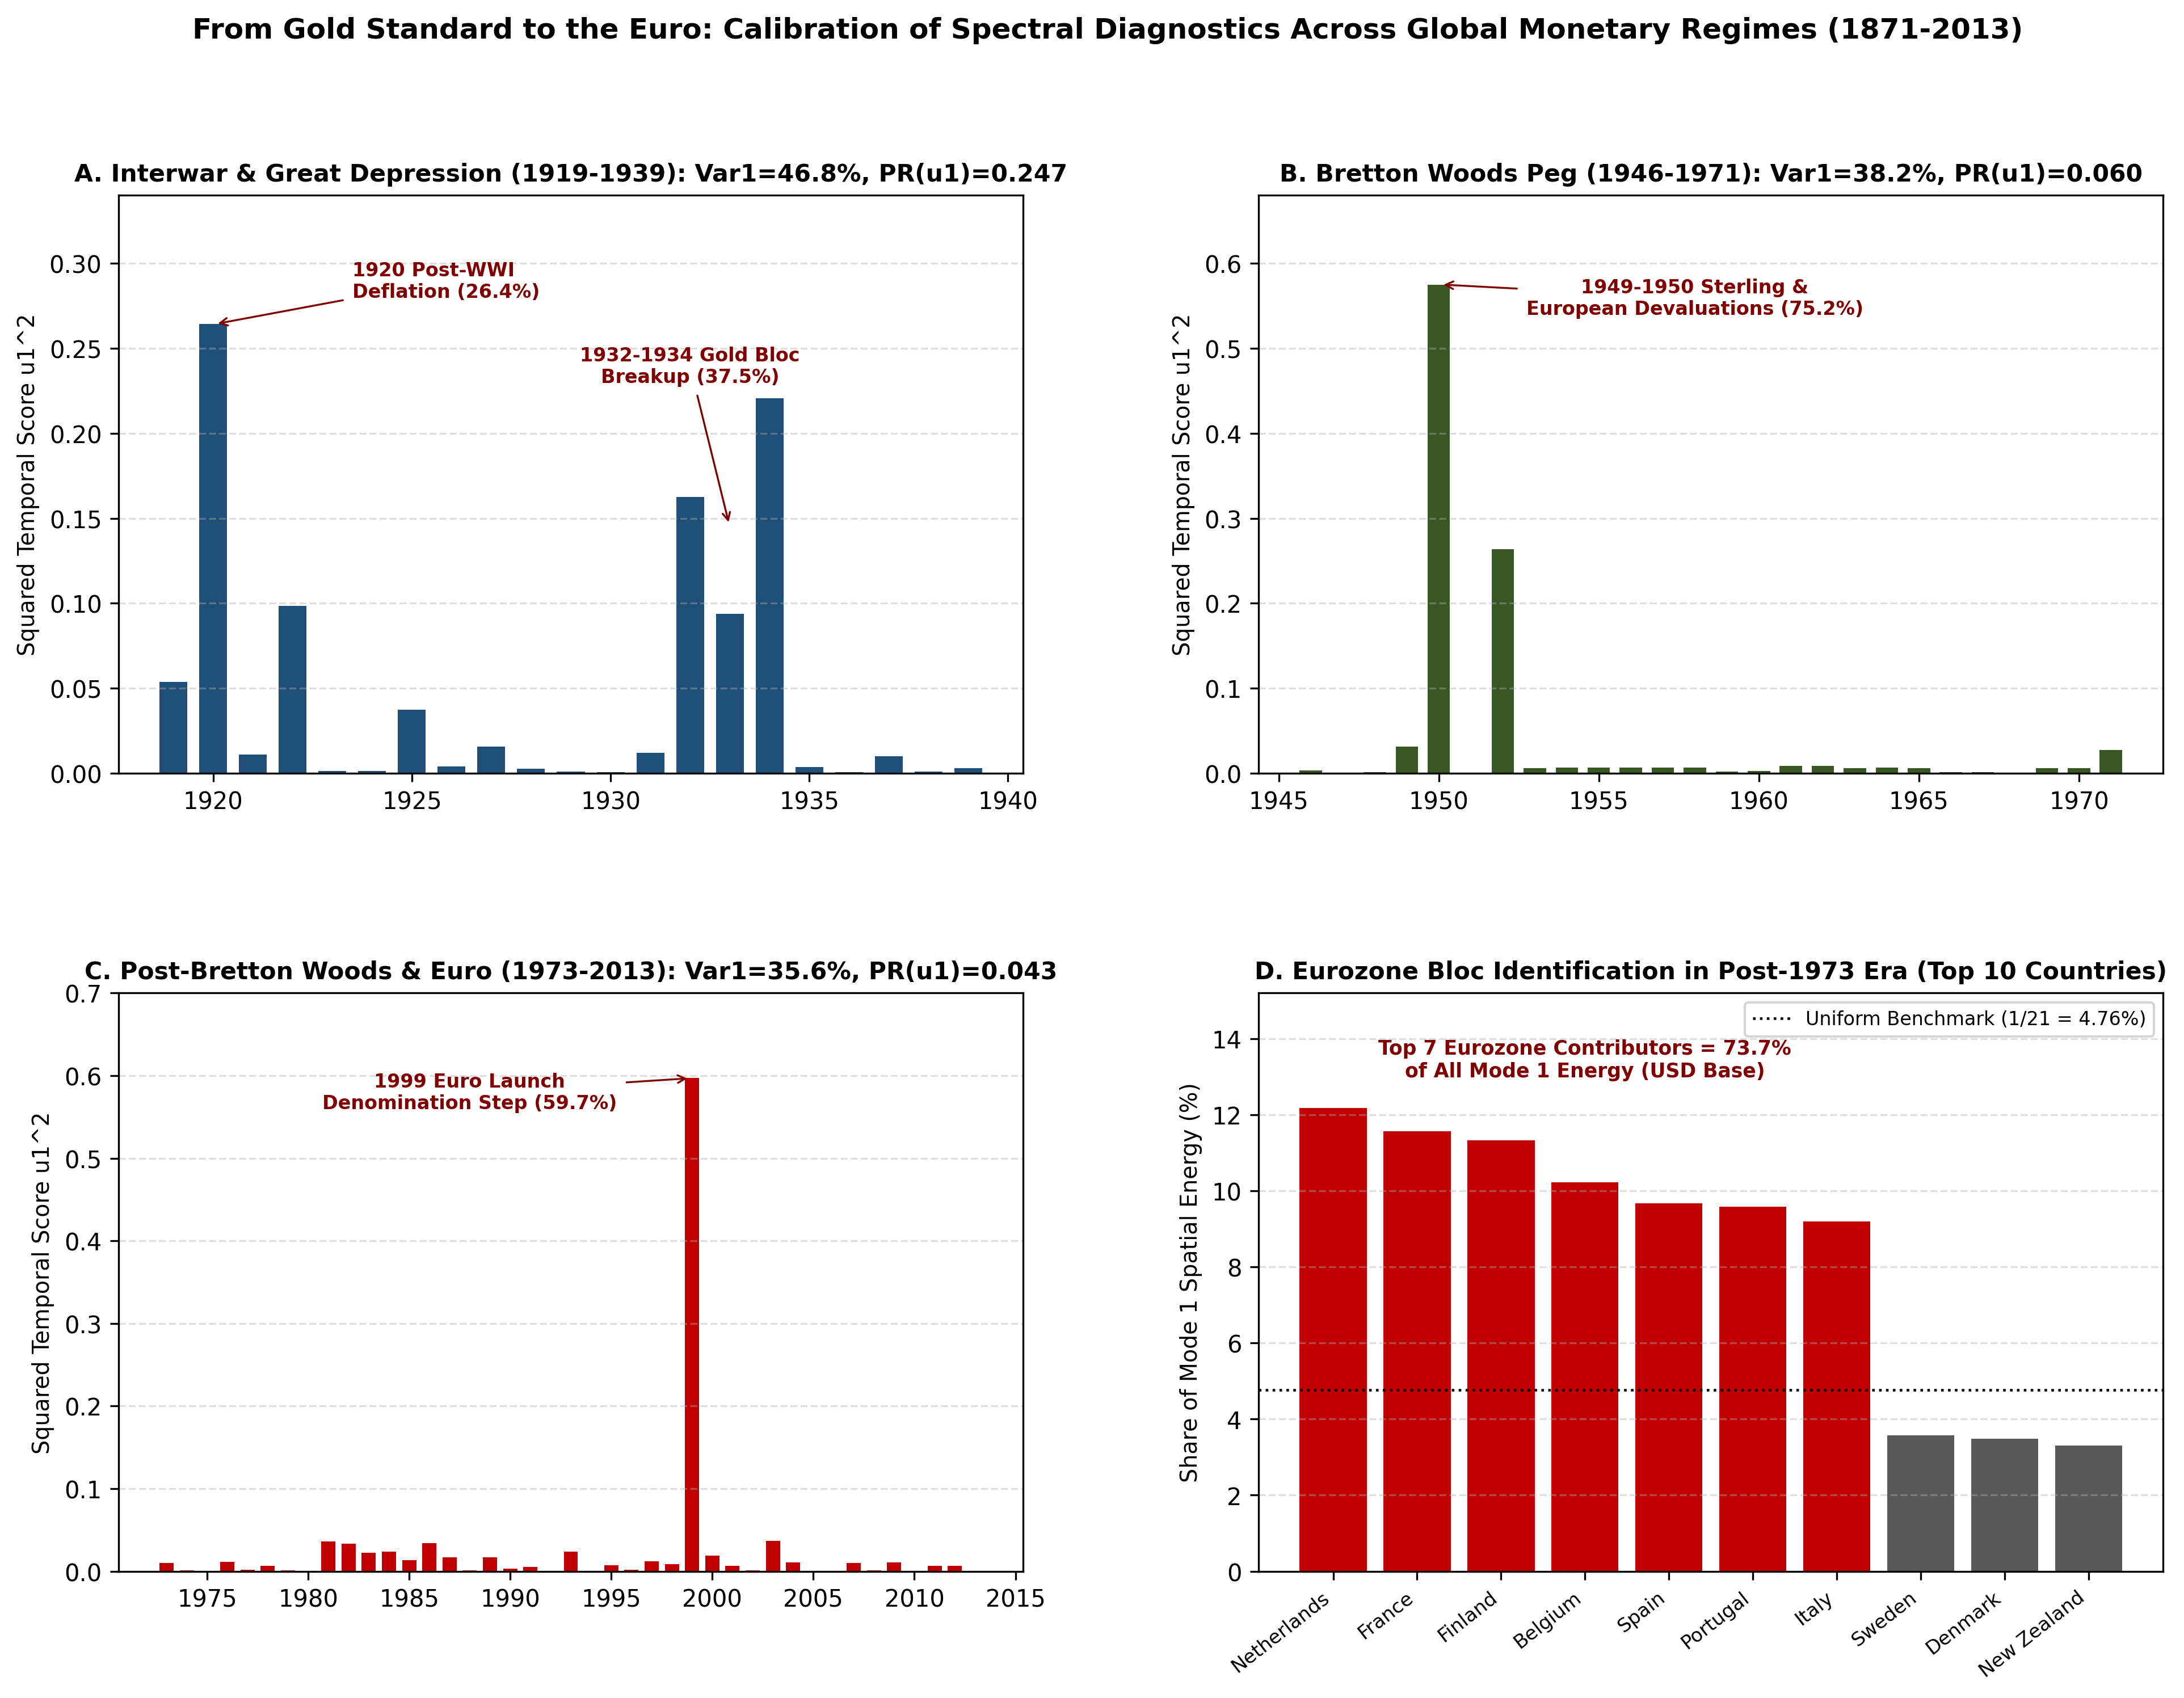
\includegraphics[width=\textwidth]{Figure_1_ModernFX.png}
\caption{\textbf{Calibration of Spectral Diagnostics Across Global Monetary Regimes (1871--2013).} \textbf{A:} Interwar temporal score energy ($u_{t,1}^2$, 1919--1939), capturing the 1920 deflation and 1932--1934 gold-bloc breakup. \textbf{B:} Bretton Woods temporal concentration (1946--1971), dominated by the 1949--1950 European devaluations (75.2 percent). \textbf{C:} Post-Bretton Woods temporal localization (1973--2013), isolating the 1999 Euro conversion step (59.7 percent). \textbf{D:} Top 10 country shares of Mode~1 spatial energy in 1973--2013, identifying the seven leading Eurozone contributors.}
\label{fig:fig1}
\end{figure}

\subsection{Post-1973 Floating Regimes and Blind Eurozone Identification}
In the post-Bretton Woods era (\texttt{1973--2013}, $M = 41$), Mode~1 accounts for 35.6 percent of global currency variance, while temporal participation drops to $\mathrm{PR}(u_1) = 0.043$ (Figure~\ref{fig:fig1}C). Nearly three-fifths of all Mode~1 temporal energy (59.7 percent in USD; 84.0 percent in GBP) occurs in the single transition of \texttt{1999}, when national European currencies were irrevocably converted into the Euro.

Remarkably, without any institutional indicators, the spatial loadings $v_1$ cleanly identify the European Monetary Union core (Figure~\ref{fig:fig1}D and Figure~\ref{fig:fig2}B). The seven largest contributors to Mode~1 spatial energy are all future Eurozone members---\texttt{Netherlands} (12.18 percent), \texttt{France} (11.56 percent), \texttt{Finland} (11.33 percent), \texttt{Belgium} (10.22 percent), \texttt{Spain} (9.67 percent), \texttt{Portugal} (9.59 percent), and \texttt{Italy} (9.19 percent)---which together capture 73.7 percent of Mode~1 variance (and 90.8 percent when measured directly against sterling), whereas \texttt{Austria} exhibits a smaller 1999 step due to its prior long-standing peg to the Deutsche Mark within the European Exchange Rate Mechanism. Meanwhile, orthogonal Mode~2 ($\mathrm{Var}_2 = 17.6$ percent; Figure~\ref{fig:fig2}B) separates emerging-market debt crises in Latin America (\texttt{Argentina}, \texttt{Brazil}, \texttt{Chile}, \texttt{Mexico}) from the European currency bloc.

\begin{figure}[htbp]
\centering
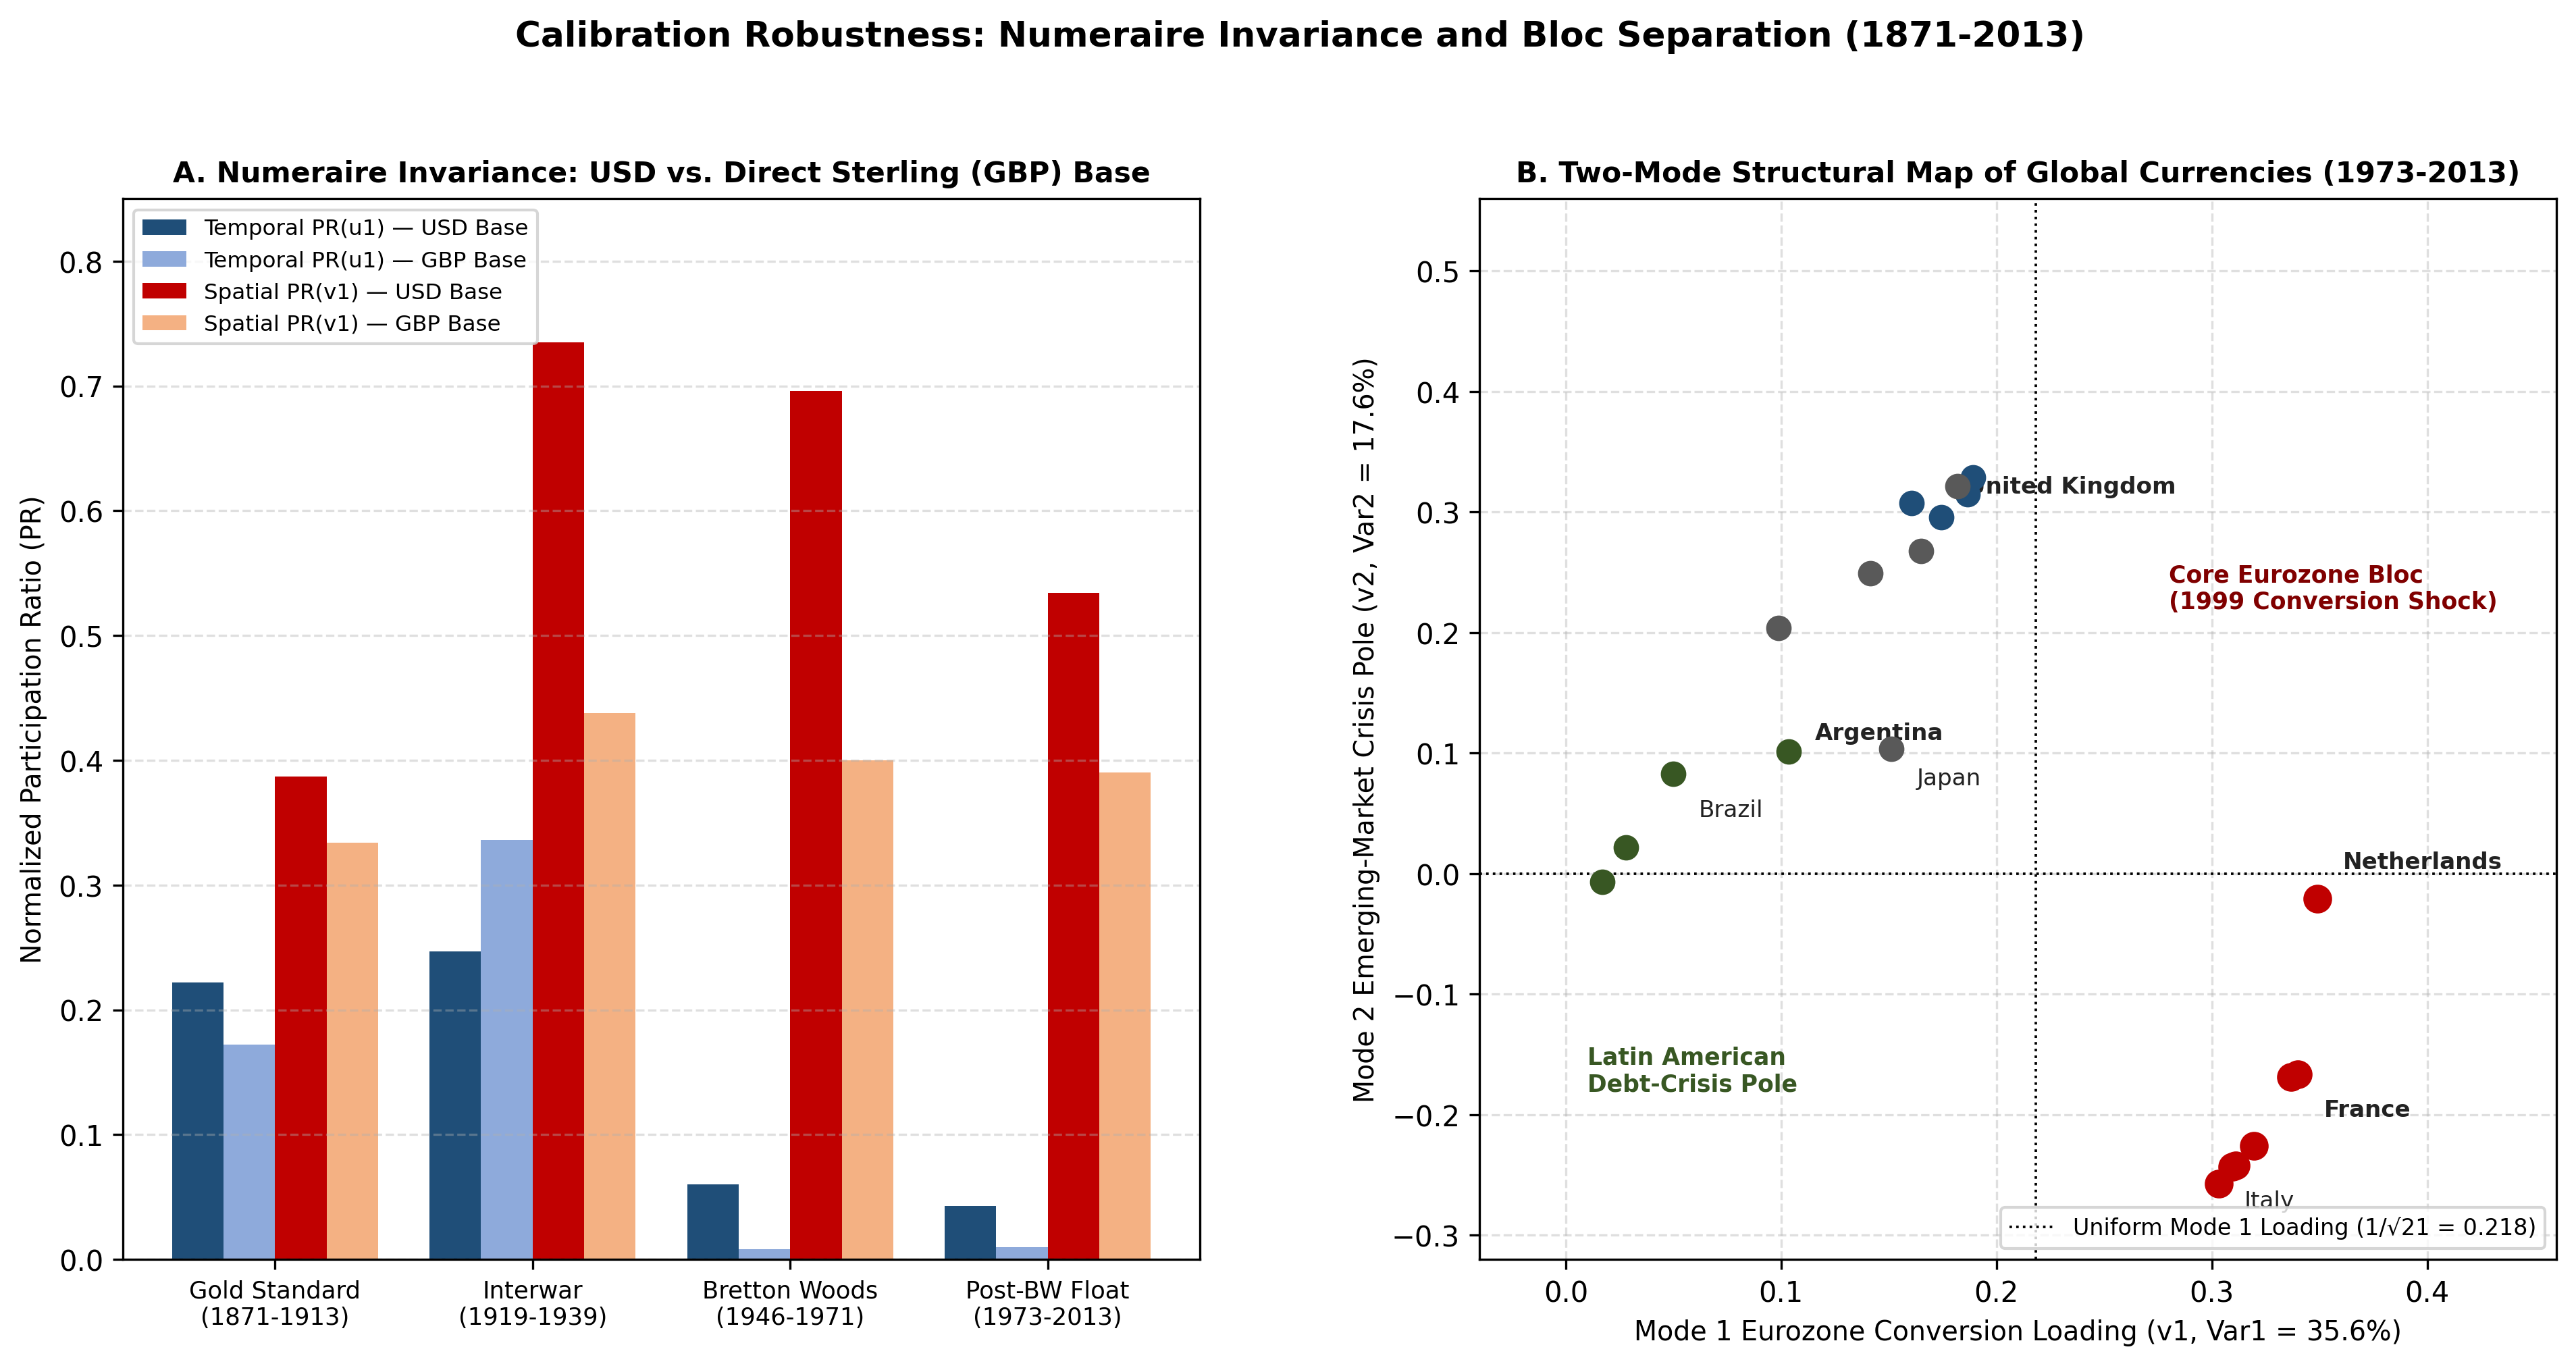
\includegraphics[width=\textwidth]{Figure_2_ModernFX.png}
\caption{\textbf{Calibration Robustness: Numeraire Invariance and Currency Bloc Separation (1871--2013).} \textbf{A:} Comparison of temporal $\mathrm{PR}(u_1)$ and spatial $\mathrm{PR}(v_1)$ across all four regimes under US dollar (USD) versus direct British pound sterling (GBP) numeraires. \textbf{B:} Two-mode structural map of all 21 currencies during the post-1973 float, separating the Eurozone bloc from non-Euro floating currencies and the Latin American debt-crisis pole.}
\label{fig:fig2}
\end{figure}

\subsection{Robustness: Numeraire Invariance and Multi-Regime Scope}
Comparing the USD-anchored panel ($N = 21$) against direct sterling quotations ($N = 20$; Table~\ref{tab:modern_fx} and Figure~\ref{fig:fig2}A) confirms that our diagnostic taxonomy is robust to the choice of anchor currency: under both numeraires, temporal localization $\mathrm{PR}(u_1)$ drops by roughly an order of magnitude when moving from the interwar float ($0.247$ USD / $0.336$ GBP) to Bretton Woods ($0.060$ USD / $0.008$ GBP) and the Euro conversion ($0.043$ USD / $0.010$ GBP).

Finally, applying our non-parametric $k$-NN transition-graph scan (Appendix~A) across the entire 143-year span (\texttt{1871--2013}) yields no single binary cut ($p > 0.59$ across all candidate years). This provides an essential methodological calibration rule: because the Fiedler eigenvector $\psi_2$ partitions a graph into two clusters, it excels at pinpointing single binary structural breaks (such as the 1857 welfare split or 1891 silver break in Eurasia; Avtonomov, 2026d), whereas multi-regime histories containing four distinct monetary eras require sub-period classification in $\big(\mathrm{PR}(u_1), \mathrm{PR}(v_1)\big)$ space.

\section{Conclusion}

Calibrating our spectral and participation-ratio toolkit against the known monetary regimes of \texttt{1870--2013} confirms that $\big(\mathrm{PR}(u_1), \mathrm{PR}(v_1)\big)$ diagnostics recover institutional currency blocs, step devaluations, and monetary unions without requiring structural break dummies or prior regime classifications. With this validation established across both early modern archives and modern international finance, the framework is ready for application to twenty-first-century commodity, energy, and geopolitical market realignments.

\section*{Data and Code Availability}
All underlying historical exchange rate series are openly accessible from Clio Infra (\url{https://clio-infra.eu}, \emph{Exchange Rates to UK Pound, 1500--2013}). Reproducible Python/Jupyter code, high-resolution figures, and LaTeX manuscript sources are openly archived on GitHub at \url{https://github.com/avtonomov-petr/From-Gold-Standard-to-the-Euro}.

\appendix
\section{Mathematical Specification of Diagnostics}
Let $E_{t,j} > 0$ denote the annual exchange rate of currency $j \in \{1,\dots,N\}$ against the anchor currency in year $t$. Within each regime window of $M$ transitions, annual log-changes $y_{t,j} = \ln E_{t,j} - \ln E_{t-1,j}$ are standardized to zero mean and unit variance, $Z_{t,j} = (y_{t,j} - \bar{y}_j)/s_j$. Thin singular value decomposition $Z = U \Sigma V^\top$ yields orthonormal temporal scores $u_1 \in \mathbb{R}^M$ and country loadings $v_1 \in \mathbb{R}^N$, with normalized participation ratios:
\begin{equation}
\mathrm{PR}(u_1) = \frac{\left(\sum_{t=1}^M u_{t,1}^4\right)^{-1} - 1}{M - 1}, \qquad
\mathrm{PR}(v_1) = \frac{\left(\sum_{j=1}^N v_{j,1}^4\right)^{-1} - 1}{N - 1}.
\end{equation}
Confidence intervals are estimated via 300 subsampling bootstrap draws without replacement at 80 percent regime length ($\lfloor 0.8M \rfloor$).

\begin{thebibliography}{99}

\bibitem{Avtonomov2026a}
Avtonomov, P. (2026a). Crisis echoes or arbitrage? Selective co-movement and integration of the Atlantic grain market, 1729--1914. \emph{Zenodo Preprint}. \url{https://doi.org/10.5281/zenodo.24436177}

\bibitem{Avtonomov2026b}
Avtonomov, P. (2026b). Blockades, flag mimicry, and grain lifelines: Physical anatomy of Russian and Baltic maritime trade in the Sound Toll Registers, 1700--1856. \emph{Zenodo Preprint}. \url{https://doi.org/10.5281/zenodo.24461586}

\bibitem{Avtonomov2026c}
Avtonomov, P. (2026c). Invisible bridges of credit: Exchange rate integration, paper assignats, and metallic anchors between St.~Petersburg and Europe, 1763--1913. \emph{Zenodo Preprint}. \url{https://doi.org/10.5281/zenodo.24498028}

\bibitem{Avtonomov2026d}
Avtonomov, P. (2026d). Eurasian continental bridges: Silver living costs, internal Russian convergence, and the Great Divergence, 1738--1913. \emph{Zenodo Preprint}. \url{https://doi.org/10.5281/zenodo.24508139}

\bibitem{Bordo1999}
Bordo, M. D., and Schwartz, A. J. (1999). Monetary policy regimes and economic performance: The historical record. In J. B. Taylor and M. Woodford (Eds.), \emph{Handbook of macroeconomics} (Vol.~1A, pp.~149--234). Elsevier.

\bibitem{Denzel2010}
Denzel, M. A. (2010). \emph{Handbook of world exchange rates, 1590--1914}. Ashgate.

\bibitem{Eichengreen2008}
Eichengreen, B. (2008). \emph{Globalizing capital: A history of the international monetary system} (2nd ed.). Princeton University Press.

\bibitem{Obstfeld2004}
Obstfeld, M., and Taylor, A. M. (2004). \emph{Global capital markets: Integration, crisis, and growth}. Cambridge University Press.

\bibitem{Reinhart2004}
Reinhart, C. M., and Rogoff, K. S. (2004). The modern history of exchange rate arrangements: A reinterpretation. \emph{Quarterly Journal of Economics}, 119(1), 1--48.

\bibitem{vanZanden2014}
van Zanden, J. L., Baten, J., Mira d'Ercole, M., Rijpma, A., Smith, C., and Timmer, M. (Eds.). (2014). \emph{How was life? Global well-being since 1820}. OECD Publishing.

\end{thebibliography}

\section*{Figure Alt Text}
\begin{itemize}
    \item \textbf{Figure 1 Alt Text:} Four-panel chart showing temporal score concentrations across the Interwar, Bretton Woods, and post-1973 eras alongside top 10 Eurozone spatial energy shares.
    \item \textbf{Figure 2 Alt Text:} Bar comparison of participation ratios under USD and GBP numeraires and two-mode scatter map separating Eurozone currencies from Latin American debt-crisis economies.
\end{itemize}

\end{document}
